\documentclass[svgnames,
               hyperref={colorlinks,citecolor=DeepPink4,linkcolor=FireBrick,urlcolor=Maroon},
               usepdftitle=false]  % see \hypersetup{} below
               {beamer}

\mode<presentation>{
  \usetheme{Madrid}
  %\usecolortheme{seagull}
  \usecolortheme{seagull}
  \setbeamercovered{transparent}
  \setbeamerfont{frametitle}{size=\large}
}

\setbeamercolor*{block title}{bg=red!10}
\setbeamercolor*{block body}{bg=red!5}

%\usepackage[svgnames]{xcolor}
\usepackage{hyperref}
\hypersetup{
    pdftitle = {Fast solvers for PDEs subject to inequalities},
    pdfauthor = {Ed Bueler and Patrick Farrell},
    pdfsubject = {},
    pdfkeywords = {}
}

\usepackage[english]{babel}
\usepackage[latin1]{inputenc}
\usepackage{times}
\usepackage[T1]{fontenc}
\usepackage{empheq,bm,xspace,fancyvrb,soul}
\usepackage{tikz}
\usetikzlibrary{shapes,arrows.meta,decorations.markings,decorations.pathreplacing,fadings,positioning}
\usepackage[kw]{pseudo}
\pseudoset{left-margin=15mm,topsep=5mm,label=,idfont=\texttt,st-left=,st-right=}

\makeatletter
%\newcommand\notsotiny{\@setfontsize\notsotiny\@vipt\@viipt}
\newcommand\notsotiny{\@setfontsize\notsotiny\@viipt\@viiipt}
\makeatother

\newcommand{\eps}{\epsilon}
\newcommand{\RR}{\mathbb{R}}

\newcommand{\grad}{\nabla}
\newcommand{\Div}{\nabla\cdot}
\newcommand{\trace}{\operatorname{tr}}

\newcommand{\hbn}{\hat{\mathbf{n}}}

\newcommand{\bb}{\mathbf{b}}
\newcommand{\be}{\mathbf{e}}
\newcommand{\bbf}{\mathbf{f}}
\newcommand{\bg}{\mathbf{g}}
\newcommand{\bn}{\mathbf{n}}
\newcommand{\bq}{\mathbf{q}}
\newcommand{\br}{\mathbf{r}}
\newcommand{\bu}{\mathbf{u}}
\newcommand{\bv}{\mathbf{v}}
\newcommand{\bw}{\mathbf{w}}
\newcommand{\bx}{\mathbf{x}}

\newcommand{\bF}{\mathbf{F}}
\newcommand{\bQ}{\mathbf{Q}}
\newcommand{\bU}{\mathbf{U}}
\newcommand{\bV}{\mathbf{V}}
\newcommand{\bX}{\mathbf{X}}

\newcommand{\btau}{\bm{\tau}}
\newcommand{\bxi}{\bm{\xi}}

\newcommand{\bzero}{\bm{0}}

\newcommand{\rhoi}{\rho_{\text{i}}}

\newcommand{\ip}[2]{\left<#1,#2\right>}

\newcommand{\nn}{{\text{n}}}
\newcommand{\pp}{{\text{p}}}
\newcommand{\qq}{{\text{q}}}
\newcommand{\rr}{{\text{r}}}

\newcommand{\ds}{\displaystyle}

\newcommand{\bus}{\bu|_s}
\newcommand{\oo}[1]{\displaystyle O\left(#1\right)}
\newcommand{\sold}{s_{\text{o}}}

\newcommand{\maxR}{R^{\bm{\oplus}}}
\newcommand{\minR}{R^{\bm{\ominus}}}
\newcommand{\iR}{R^{\bullet}}


\title[Fast solvers for PDE+inequalities]{Fast solvers for partial differential equations \\ subject to inequalities}

%\subtitle{\emph{}}

\author[Bueler and Farrell]{Ed Bueler \inst{1} \and Patrick Farrell \inst{2}}
\institute[]{\inst{1} University of Alaska Fairbanks \and %
             \inst{2} Mathematical Institute, Oxford University}

\date[]{November 2023}

%\titlegraphic{\begin{picture}(0,0)
%    \put(0,180){\makebox(0,0)[rt]{\includegraphics[width=4cm]{figs/software.png}}}
%  \end{picture}
%}

\titlegraphic{\vspace{-8mm} 
\includegraphics[width=0.26\textwidth]{../talk-oxford/images/uafbw.png} \hfill \begin{minipage}{0.14\textwidth}

\includegraphics[width=\textwidth]{../talk-oxford/images/oxford.png}

\vspace{18mm}
\end{minipage} \vspace{-10mm}}

%% to start section counter at 0 see
%% https://tex.stackexchange.com/questions/170222/change-the-numbering-in-beamers-table-of-content


\begin{document}
\beamertemplatenavigationsymbolsempty

{
  %\usebackgroundtemplate{\includegraphics[width=\paperwidth]{../talk-oxford/images/gray-british-clark2022.png}}
  \begin{frame}
    \titlepage
  \end{frame}
}

\begin{frame}{Outline}
  \tableofcontents[hideallsubsections]
  %\tableofcontents

%\vfill
%{\footnotesize \emph{PDEs = partial differential equations}}
\end{frame}


\section{variational inequalities (VIs)}

\begin{frame}{example: classical obstacle problem}

\begin{center}
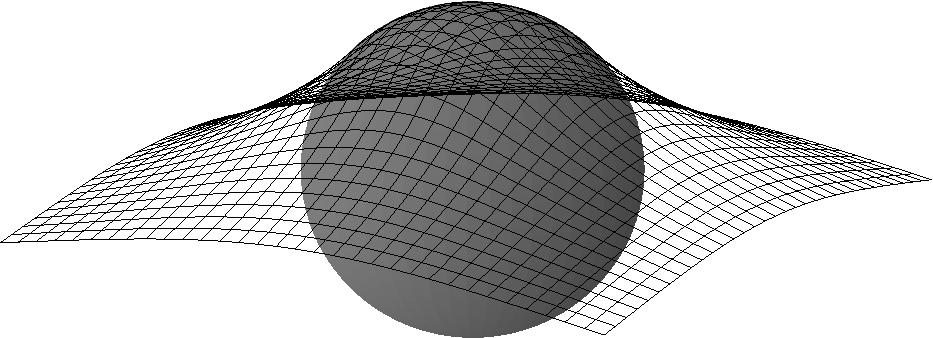
\includegraphics[width=0.65\textwidth]{../talk-oxford/images/obstacle65.pdf}
\end{center}

\only<1-2>{
\begin{itemize}
\item \emph{problem.} on a domain $\Omega \subset \RR^2$, find the displacement $u(x)$ of a membrane, with fixed value $u = g$ on $\partial \Omega$, above an \emph{obstacle} $\psi(x)$, which minimizes elastic (plus some potential) energy
    $$J(v) = \int_\Omega \frac{1}{2} |\grad v|^2 - f\, v$$
\item shown above: \quad $\Omega$ a square, $\psi(x)$ a hemisphere
\item<2>[\alert{Q.}] how to solve this as a PDE with boundary conditions?
\end{itemize}

\vspace{2mm}
}
\only<3>{
\begin{itemize}
\item this is constrained optimization over an infinite-dimensional \emph{admissible set}
	$$\mathcal{K} = \left\{v \in H^1(\Omega) \,:\, v\big|_{\partial \Omega} = g \,\text{ and }\, v \ge \psi\right\}$$

    \begin{itemize}
    \item[$\circ$] $\mathcal{K}$ is a closed and convex subset of the Sobolev space
   $$H^1(\Omega) = \left\{v \,:\, \int_\Omega |v|^2 + |\grad v|^2 < \infty\right\}$$
    \end{itemize}
\end{itemize}
}
\end{frame}


\begin{frame}{example: classical obstacle problem}

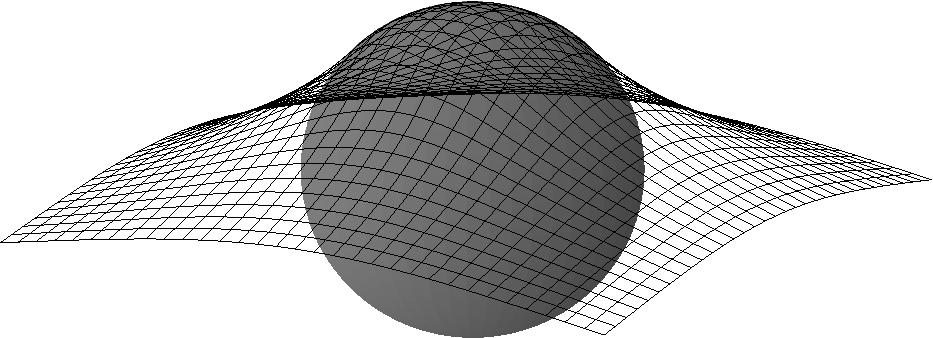
\includegraphics[width=0.55\textwidth]{../talk-oxford/images/obstacle65.pdf} \qquad 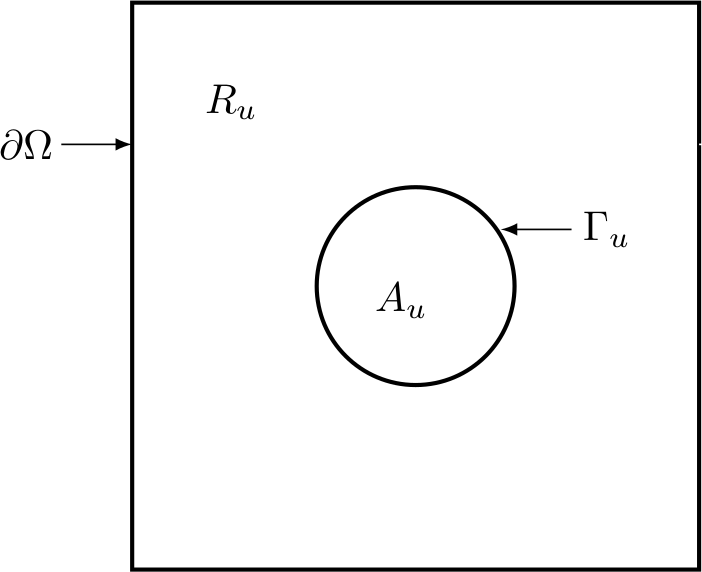
\includegraphics[width=0.35\textwidth]{../talk-oxford/images/obstacle-sets.png}

\bigskip
\only<1>{
\begin{itemize}
\item the solution defines subsets of $\Omega$:
   \begin{itemize}
   \item[$\circ$] \emph{active set} $A_u = \{u = \psi\}$
   \item[$\circ$] \emph{inactive set} $R_u = \{u> \psi\}$
   \item[$\circ$] \emph{free boundary} $\Gamma_u=\partial R_u \cap \Omega$
   \end{itemize}
\end{itemize}

\vspace{25mm}
}
\only<2-3>{
\begin{itemize}
\item a naive strong form would pose the problem in terms of its solution:
\begin{align*}
-\grad^2 u &= f \quad \text{ on $R_u$} \\
u &= \psi \quad \text{ on $A_u$}
\end{align*}

   \begin{itemize}
   \item[$\circ$] Poisson equation $-\grad^2 u = f$ is ``$J'(u)=0$'' on $R_u$
   \item<3>[$\circ$] using the solution $u$ to define the set $R_u$ on which to solve the PDE $-\grad^2 u = f$ \alert{does not lead to solution algorithms}
   \end{itemize}
\end{itemize}
}
\only<4>{
\begin{itemize}
\item the \emph{complementarity problem} (CP) is a meaningful strong form:
\begin{align*}
u - \psi &\ge 0 \\
-\grad^2 u - f &\ge 0 \\
(u - \psi)(-\grad^2 u - f) &= 0
\end{align*}

   \begin{itemize}
   \item[$\circ$] CP $=$ (KKT conditions in $\infty$-dimensions)
   \end{itemize}

\phantom{x}

\phantom{x}
\end{itemize}
}
\only<5>{
\begin{itemize}
\item the weak form is a {\color{FireBrick} \emph{variational inequality} (VI)}, which says that $J'(u)$ points directly into $\mathcal{K}$:
    $$\ip{J'(u)}{v-u} = \int_\Omega \grad u\cdot \grad (v-u) - f (v-u) \ge 0$$
for all $v \in \mathcal{K}$

\vspace{11mm}
\end{itemize}
}
\end{frame}


\begin{frame}{VI $=$ weak form with $v-u$ as the test function}

{\small
   $$J(u) \le J(v) \quad \forall v \in \mathcal{K} \qquad \iff \qquad \ip{J'(u)}{v-u} \ge 0 \quad \forall v \in \mathcal{K}$$
}

\bigskip
\begin{center}
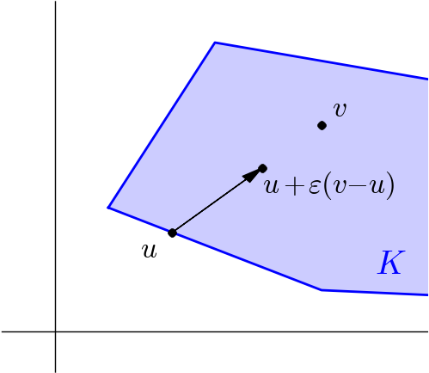
\includegraphics[width=0.5\textwidth]{figs/convexuv.png}
\end{center}
\end{frame}



\begin{frame}{general variational inequalities}

\begin{itemize}
\item let $\mathcal{K}$ be a closed and convex subset of a Banach space $\mathcal{V}$
\item suppose $F:\mathcal{K} \to \mathcal{V}'$ is a continuous operator
    \begin{itemize}
    \item[$\circ$] $F$ is generally nonlinear
    \item[$\circ$] $F$ may be defined \emph{only} on $\mathcal{K}$
    \item[$\circ$] $F$ may \emph{not}\, be the derivative of an objective function $J$
    \item[$\circ$] $F=J'$, a linear operator, in classical obstacle problem
    \end{itemize}
\item the general variational inequality {\color{FireBrick} VI($F$,$\mathcal{K}$)} is
	$${\color{FireBrick} \ip{F(u)}{v-u} \ge 0 \quad \text{ for all } v \in \mathcal{K}}$$
\item when $\mathcal{K}$ is nontrivial the problem {\color{FireBrick} VI($F$,$\mathcal{K}$)} is nonlinear \emph{even when $F$ is a linear operator}
\end{itemize}
\end{frame}


\begin{frame}{VI $=$ constrained ``system of equations''}

\begin{center}
\begin{tabular}{r|l|l}
& \qquad unconstrained & \qquad constrained \\ \hline
optimization &
\begin{minipage}[t][16mm][t]{0.32\textwidth}
$$\min_{u\in\mathcal{V}} J(u)$$
\end{minipage}
&
\begin{minipage}[t][16mm][t]{0.35\textwidth}
$$\min_{u\in\mathcal{K} \subset \mathcal{V}} J(u)$$
\end{minipage}
\\ \hline
\only<1>{equations}\only<2>{\begin{minipage}[t][16mm][t]{0.15\textwidth} weak form \par equations \end{minipage}} &
\begin{minipage}[t][16mm][t]{0.32\textwidth}

\vspace{-2mm}
find $u \in \mathcal{V}$:
\only<1>{$$F(u)=0$$}
\only<2>{$$\ip{F(u)}{v} = 0 \quad \forall v \in \mathcal{V}$$}
\end{minipage}
&
\begin{minipage}[t][16mm][t]{0.35\textwidth}

\vspace{-2mm}
find $u \in \mathcal{K} \subset \mathcal{V}$:
$${\color{FireBrick} \ip{F(u)}{v-u} \ge 0 \quad \forall v \in \mathcal{K}}$$
\end{minipage}
\end{tabular}
\end{center}
\end{frame}


\begin{frame}{applications of VIs}

\begin{itemize}
\item elastic contact
    \begin{itemize}
    \item[$\circ$] car tires, for example
    \end{itemize}

\vspace{-10mm}
\hfill 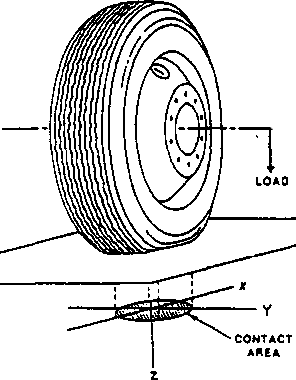
\includegraphics[width=0.2\textwidth]{figs/tirecontact.png}

\vspace{-20mm}
\item pricing of American options
    \begin{itemize}
    \item[$\circ$] inequality-constrained Black-Scholes model
    \end{itemize}

\vspace{1.5mm}
\item the geometry of glaciers %\hfill $\longleftarrow$ \emph{more soon}

\vspace{3mm}
\item first-semester calculus:
    $$u \gets \min_{x\in[a,b]} f(x) \quad \iff \quad f'(u)(v-u) \ge 0 \quad \forall v \in[a,b]$$
\end{itemize}

%\vspace{20mm}
\begin{center}
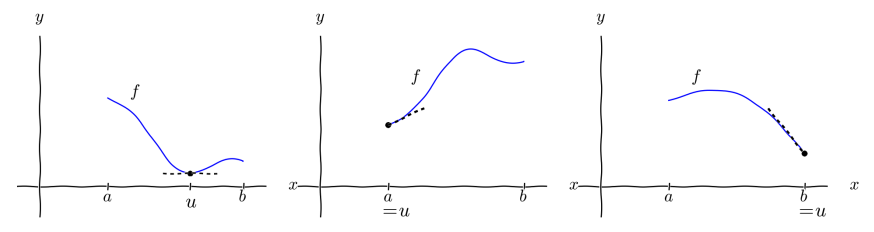
\includegraphics[width=0.9\textwidth]{../talk-oxford/images/calcone.png}
\end{center}
\end{frame}


\AtBeginSection[]
{
  \begin{frame}{Outline}
    \tableofcontents[currentsection]
  \end{frame}
}

\section{nonlinear multigrid for PDEs}

\subsection{full approximation scheme (FAS)}

\begin{frame}{nonlinear 2-mesh scheme}

\begin{center}
$\Omega^h$\, 
\includegraphics[height=0.16\textheight]{../talk-oxford/images/fine-grid.png} \hspace{25mm} 
\includegraphics[height=0.16\textheight]{../talk-oxford/images/coarse-grid.png} \,$\Omega^H$
\end{center}

\only<1>{
\begin{itemize}
\item consider a nonlinear elliptic PDE problem:
	$$F(u) = \ell$$

	\begin{itemize}
	\item[$\circ$] $u\in \mathcal{V}=H^1(\Omega)$
	\item[$\circ$] $\ell\in \mathcal{V}'$
	\item[$\circ$] $F : \mathcal{V} \to \mathcal{V}'$ continuous and injective
	\item[$\circ$] for example, the Liouville-Bratu problem: $-\grad^2 u - e^u = f$
	\end{itemize}
\item discretization gives algebraic system on fine mesh $\Omega^h$:
    $$F^h(u^h) = \ell^h$$

	\begin{itemize}
	\item[$\circ$] $u^h$ denotes exact (algebraic) solution
	\end{itemize}
\end{itemize}

\vspace{4mm}
}
\only<2-3>{
\begin{itemize}
\item \emph{goal}: to solve $F^h(u^h) = \ell^h$ on $\Omega^h$
\item suppose $w^h$ is a not-yet-converged iterate:
    $$r^h=\ell^h - F^h(w^h), \qquad \|r^h\| > \text{TOL}$$
\item how can we improve $w^h$ \emph{without} globally linearizing $F^h$?

	\begin{itemize}
	\item are there alternatives to Newton's method?
	\end{itemize}
\item<3> notes:
    \setbeamertemplate{enumerate item}{\emph{\roman{enumi})}}
    \begin{enumerate}
    \item the \emph{residual} \quad $r^h = \ell^h - F^h(w^h)$ \quad is computable
    \item the \emph{error} \quad $e^h = u^h-w^h$ \quad is unknown
    \item our equation can be rewritten
    $$F^h(u^h) - F^h(w^h) = r^h$$
    \end{enumerate}
\end{itemize}
}
\only<4-5>{
\begin{itemize}
\item \emph{updated goal}: from iterate $w^h$, to solve
    $$F^h(u^h) - F^h(w^h) = r^h$$
\item \alert{for $F^h$ linear}, convert this to the \emph{error equation}
    $$F^h(e^h) = r^h$$
\item an approximation solution $\tilde e^h$ would improve our iterate:
    $$w^h \leftarrow w^h+\tilde e^h$$
\item<5> but $F^h$ is not linear!
\end{itemize}

\vspace{5mm}
}
\only<6>{
\begin{itemize}
\item \emph{updated goal}: use a coarser mesh $\Omega^H$ to somehow estimate the solution $u^h$ in the nonlinear \emph{correction equation}
    $${\color{FireBrick} F^h(u^h) - F^h(w^h) = r^h}$$
\item basic multigrid idea: there are algorithms (\alert{smoothers}) which ``improve'' $w^h$ \dots use them a little first \dots then correct from the coarser mesh
    \begin{itemize}
    \item[$\circ$] ``improve'' means they remove high-frequency error components efficiently
    \end{itemize}
\end{itemize}

\vspace{15mm}
}
\only<7>{
\begin{itemize}
\item \emph{nodewise problem}: for $\psi_i^h$ a hat function or dof, solve for $c\in\RR$ to make the residual at that location zero:
	$${\color{FireBrick} \phi_i(c) = r^h(w^h + c \psi_i^h)[\psi_i^h] = 0}$$
\item sweeping through and solving nodewise problems is a \alert{smoother}
    \begin{itemize}
    \item[$\circ$] Fourier analysis shows smoothing property
    \item[$\circ$] after smoothing, $e^h$ and $r^h$ have smaller high-frequencies
    \end{itemize}
\item after smoothing, the correction equation on $\Omega^h$ should be accurately approximate-able on the coarser mesh $\Omega^H$
\end{itemize}

\vspace{14mm}
}
\only<8-9>{
\begin{itemize}
\item \emph{updated goal}: use a coarser mesh $\Omega^H$ to somehow estimate the solution $u^h$ in $F^h(u^h) - F^h(w^h) = r^h(w^h)$
\item Brandt's (1977) \emph{full approximation scheme} (FAS) equation:
	$${\color{FireBrick} F^H(u^H) - F^H(\iR w^h) = R \, r^h(w^h)}$$

    \begin{itemize}
    \item[$\circ$] $\iR:\mathcal{V}^h \to \mathcal{V}^H$ is node-wise \emph{injection}
    \item[$\circ$] $R:(\mathcal{V}^h)' \to (\mathcal{V}^H)'$ is \emph{canonical restriction}
    \item[$\circ$] note: if $w^h=u^h$ exactly then $u^H = \iR w^h$ since $F^H$ injective
    \end{itemize}

\item<9> rewritten FAS equation: let ${\color{FireBrick} \ell^H = F^H(\iR w^h) + R\, r^h(w^h)}$ then
    $${\color{FireBrick} F^H(u^H) = \ell^H}$$
\end{itemize}

\vspace{-3mm}
}
\end{frame}


\begin{frame}{full approximation scheme (FAS) 2-mesh solver}

\begin{center}
fine mesh $=\Omega^h$\, 
\includegraphics[height=0.14\textheight]{../talk-oxford/images/fine-grid.png} \hspace{15mm} 
\includegraphics[height=0.14\textheight]{../talk-oxford/images/coarse-grid.png} \,$\Omega^H=$ coarse mesh
\end{center}

\begin{align*}
&\text{pre-smooth over fine:} & & [\text{smoother updates } w^h] \\
&\text{\textbf{restrict}:}                   & &\ell^H = F^H(\iR w^h) + R\, r^h(w^h) \\
&\text{\textbf{solve coarse}:}                      & &F^H(w^H) = \ell^H \\
&\text{\textbf{correct}:}                    & &w^h \leftarrow w^h + P(w^H - \iR w^h) \\
&\text{post-smooth over fine:} & & [\text{smoother updates } w^h]
\end{align*}

\bigskip
{\small
\begin{itemize}
\item $P: \mathcal{V}^H \to \mathcal{V}^h$ is \emph{canonical prolongation}
\item \textbf{restrict}$+$(\textbf{solve coarse})$+$\textbf{correct} \, $=$ \, \emph{FAS coarse grid correction}
\end{itemize}
}
\end{frame}


\begin{frame}{nonlinear multigrid by FAS: \only<1>{V-cycle}\only<2>{FMG cycle}}

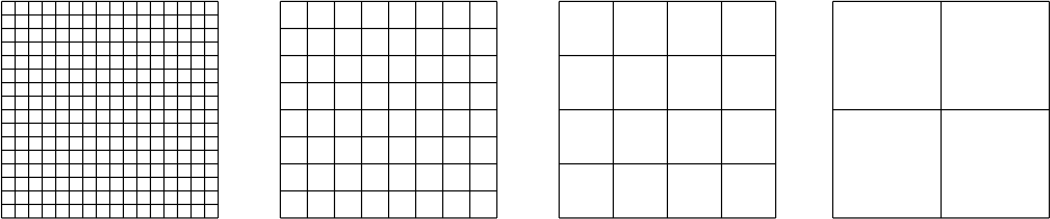
\includegraphics[height=0.2\textheight]{../talk-oxford/images/mg-grids.png}

\hspace{4mm} $J=3$ \hspace{13mm} $j=2$ \hspace{13mm} $j=1$ \hspace{12mm} $j=0$

\bigskip
\only<1>{
\begin{columns}
\begin{column}{0.75\textwidth}
{\small
\begin{pseudo}
\pr{fas-vcycle}$(\ell^J;w^J)$: \\+
    for $j=J$ downto $j=1$ \\+
      $\text{\pr{smooth}}^{\text{\id{down}}}(\ell^j; w^j)$ \\
      $w^{j-1} = \iR w^j$ \\
      $\ell^{j-1} = F^{j-1}(w^{j-1}) + R \left(\ell^j - F^j(w^j)\right)$ \\-
    $\text{\pr{solve}}(\ell^0;w^0)$ \\
    for $j=1$ to $j=J$ \\+
      $w^j \gets w^j + P (w^{j-1} - \iR w^j)$ \\
      $\text{\pr{smooth}}^{\text{\id{up}}}(\ell^j;w^j)$ \\-
\end{pseudo}
}
\end{column}
\begin{column}{0.25\textwidth}
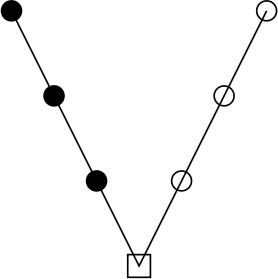
\includegraphics[width=0.7\textwidth]{../talk-oxford/images/mg-vcycle.png}
\end{column}
\end{columns}
}
\only<2>{
\vspace{6mm}

\centering
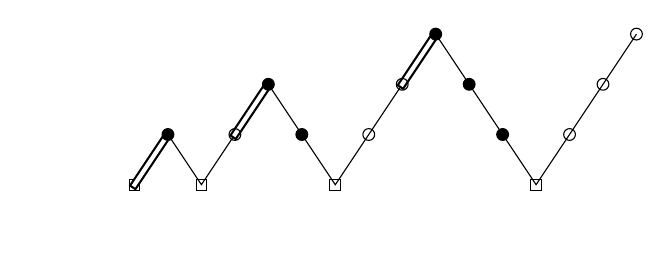
\begin{tikzpicture}[scale=0.85]
  \pgfmathsetmacro\hstep{0.5}
  \pgfmathsetmacro\vstep{0.75}
  \pgfmathsetmacro\ceps{0.08}   % size of square for coarse grid

% initial restriction to coarsest
  \pgfmathsetmacro\hoff{0*\hstep}
  %\draw[shift={(\hoff,0)},gray,line width=1.0mm] (0.0,3*\vstep) -- (\hstep,2*\vstep) --  (2*\hstep,\vstep) -- (3*\hstep,0.0);
  \draw[shift={(\hoff,0)}]     (3*\hstep-\ceps,-\ceps) rectangle (3*\hstep+\ceps,+\ceps);
  \draw[shift={(\hoff,0)},black,thick,double,double distance between line centers=0.8mm,line cap=rect] (3*\hstep,0.0) -- (4*\hstep,\vstep);

% V-cycle to level 1
  \pgfmathsetmacro\hoff{4*\hstep}
  \draw[shift={(\hoff,0)},black,thin] (0.0,\vstep) -- (\hstep,0.0) -- (2*\hstep,\vstep);
  \draw[shift={(\hoff,0)},black,thick,double,double distance between line centers=0.8mm,line cap=rect] (2*\hstep,\vstep) -- (3*\hstep,2*\vstep);
  \filldraw[shift={(\hoff,0)}] (0.0,\vstep) circle (2.5pt);
  \draw[shift={(\hoff,0)}]     (\hstep-\ceps,-\ceps) rectangle (\hstep+\ceps,+\ceps);
  \draw[shift={(\hoff,0)}]     (2*\hstep,\vstep) circle (2.5pt);

% V-cycle to level 2
  \pgfmathsetmacro\hoff{7*\hstep}
  \draw[shift={(\hoff,0)},black,thin] (0.0,2*\vstep) --  (\hstep,\vstep) -- (2*\hstep,0.0) -- (3*\hstep,\vstep) -- (4*\hstep,2*\vstep);
  \draw[shift={(\hoff,0)},black,thick,double,double distance between line centers=0.8mm,line cap=rect] (4*\hstep,2*\vstep) -- (5*\hstep,3*\vstep);
  \filldraw[shift={(\hoff,0)}] (0.0,2*\vstep) circle (2.5pt);
  \filldraw[shift={(\hoff,0)}] (\hstep,\vstep) circle (2.5pt);
  \draw[shift={(\hoff,0)}]     (2*\hstep-\ceps,-\ceps) rectangle (2*\hstep+\ceps,+\ceps);
  \draw[shift={(\hoff,0)}]     (3*\hstep,\vstep) circle (2.5pt);
  \draw[shift={(\hoff,0)}]     (4*\hstep,2*\vstep) circle (2.5pt);

% V-cycle to finest (level 3)
  \pgfmathsetmacro\hoff{12*\hstep}
  \draw[shift={(\hoff,0)},black,thin] (0.0,3*\vstep) -- (\hstep,2*\vstep) --  (2*\hstep,\vstep) -- (3*\hstep,0.0) -- (4*\hstep,\vstep) -- (5*\hstep,2*\vstep) -- (6*\hstep,3*\vstep);
  \filldraw[shift={(\hoff,0)}] (0.0,3*\vstep) circle (2.5pt);
  \filldraw[shift={(\hoff,0)}] (\hstep,2*\vstep) circle (2.5pt);
  \filldraw[shift={(\hoff,0)}] (2*\hstep,\vstep) circle (2.5pt);
  \draw[shift={(\hoff,0)}]     (3*\hstep-\ceps,-\ceps) rectangle (3*\hstep+\ceps,+\ceps);
  \draw[shift={(\hoff,0)}]     (4*\hstep,\vstep) circle (2.5pt);
  \draw[shift={(\hoff,0)}]     (5*\hstep,2*\vstep) circle (2.5pt);
  \draw[shift={(\hoff,0)}]     (6*\hstep,3*\vstep) circle (2.5pt);

  \draw[white] (0, -\vstep) circle (2.5pt);
\end{tikzpicture}



FMG $=$ full multigrid

\vspace{6mm}
}
\end{frame}


\begin{frame}{does it work?}

\begin{itemize}
\item FAS multigrid works \alert{very well} on nice nonlinear PDE problems
\item example: Liouville-Bratu equation
    $$-\nabla^2 u - e^u = 0$$
with Dirichlet boundary conditions on $\Omega=(0,1)^2$
\item discretize by (straightforward) finite differences
\item minimal problem-specific code:
    \begin{enumerate}
    \item[1.] residual evaluation on grid level: $F^j(\cdot)$
    \item[2.] pointwise smoother: $\phi_i(c) = 0 \,\forall i$
        \begin{itemize}
        \item[$\circ$] nonlinear Gauss-Seidel iteration
        \end{itemize}
    \item[3.] coarsest-level solve can be same as smoother, or more sophisticated (e.g.~Newton iteration)
    \end{enumerate}
\end{itemize}
\end{frame}


\begin{frame}{the meaning of ``fast solver''}

\begin{itemize}
\item what does ``very well'' on the previous slide mean?
\end{itemize}

\begin{block}{definition} a solver is \emph{optimal} if work in flops, and/or run-time, is $O(N)$ for $N$ unknowns
\end{block}

\begin{itemize}
\item since $\sim$1980: optimality can be achieved by multigrid for PDE problems with reasonably-smooth solutions
\item<2> in fact, multigrid people get greedy
\end{itemize}

\begin{block}<2>{definition} a solver exhibits \emph{textbook multigrid efficiency} if it is optimal and it does total work less than 10 times that of a single smoother sweep
\end{block}
\end{frame}


\begin{frame}{Bratu model problem: optimality and TME}

\begin{columns}
\begin{column}{0.45\textwidth}
\begin{itemize}
\item \texttt{bratu.c}
\item observed optimality:
\begin{align*}
\text{flops} &= O(N^1) \\
\text{exp evaluations} &= O(N^1) \\
\text{processor time} &= O(N^1)
\end{align*}
\item {\color{FireBrick} $12$-level V-cycle} has $N\approx 10^8$ unknowns
\item compare $\approx 20\,\mu\,\text{s}/\text{N}$ for Poisson using Firedrake ($P_1$, geometric multigrid)
\end{itemize}
\end{column}
\begin{column}{0.55\textwidth}
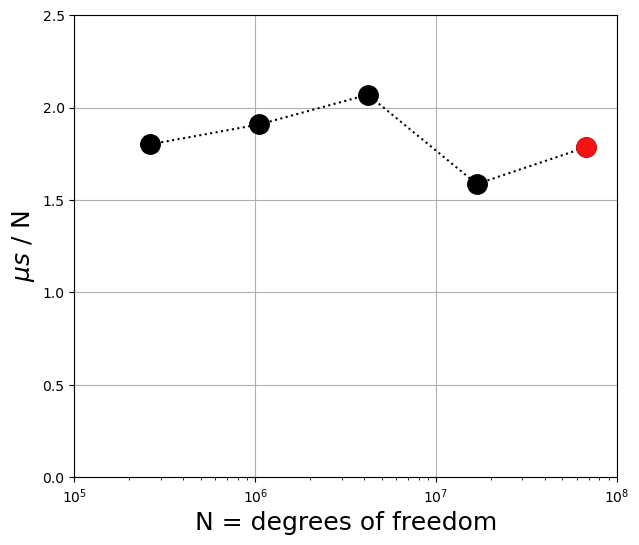
\includegraphics[width=\textwidth]{figs/bratu-time.png}
\end{column}
\end{columns}
\end{frame}


\section{multigrid for VIs}

\subsection{an earlier approach}

\begin{frame}[fragile]
\frametitle{Newton-multigrid for the classical obstacle problem}

\begin{itemize}
\item best-known multigrid method for VIs: Newton-multigrid
    \begin{itemize}
    \item[$\circ$] linear solver applies to currently-inactive variables
        \begin{itemize}
        \item ``reduced space line search''
        \end{itemize}
    \item[$\circ$] Newton step equations solved by CG with linear multigrid V-cycles
    \end{itemize}
\item observed in actual use: grid-dependent Newton iterations
\item the (outer) Newton iteration must converge on the active set \alert{before} linear multigrid can provide effective preconditioning
\end{itemize}

\medskip
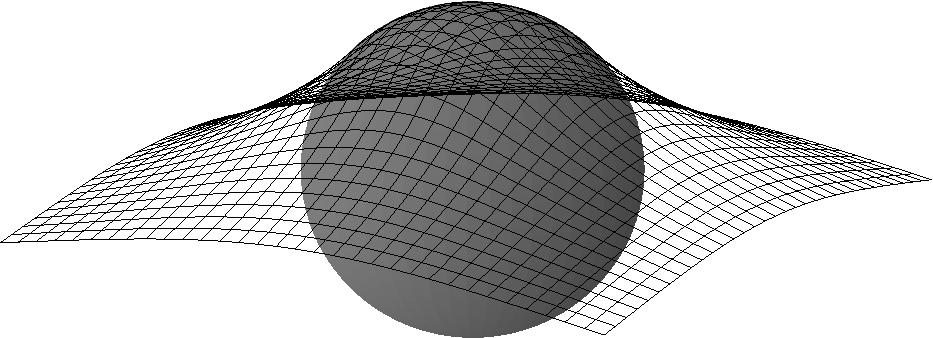
\includegraphics[height=0.15\textheight]{../talk-oxford/images/obstacle65.pdf} \qquad 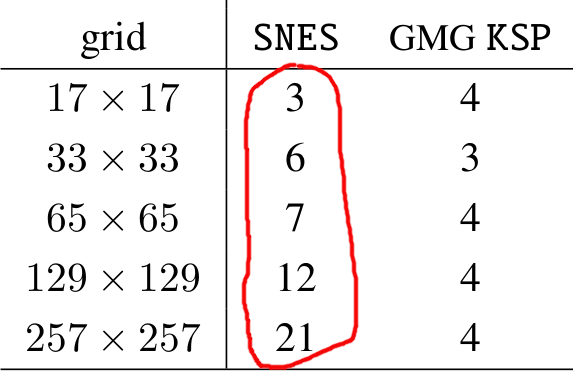
\includegraphics[height=0.25\textheight]{../talk-oxford/images/vi-newton-gmg-bad.png}
\end{frame}


\begin{frame}[fragile]
\frametitle{nested iteration}

\begin{itemize}
\item on simpler VI problems, \alert{nested iteration} helps
    \begin{itemize}
    \item[$\circ$] nested-iteration = grid-sequencing
    \item[$\circ$] on classical obstacle problem: mesh-independent Newton iterations, optimal $O(N)$ flops and time; Chapter 12 in my book
    \end{itemize}
\item not as effective on harder (\emph{lower-regularity, complicated free boundary}) problems
\end{itemize}

\medskip
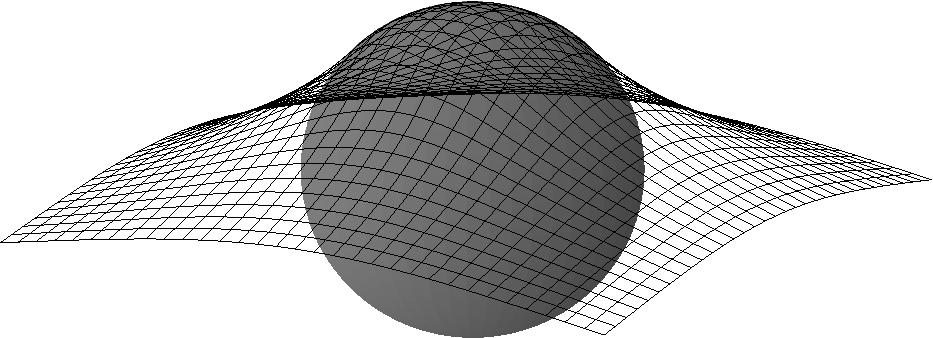
\includegraphics[height=0.15\textheight]{../talk-oxford/images/obstacle65.pdf} \qquad 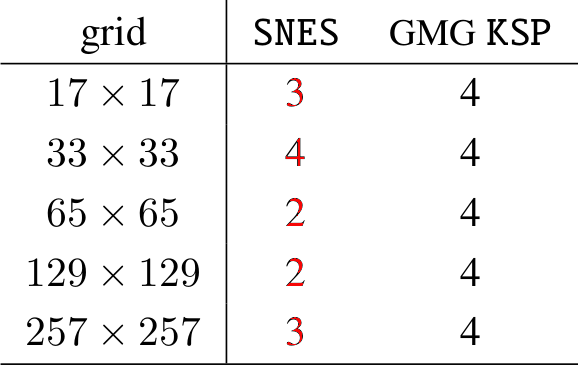
\includegraphics[height=0.25\textheight]{../talk-oxford/images/vi-newton-gmg-good.png} \qquad 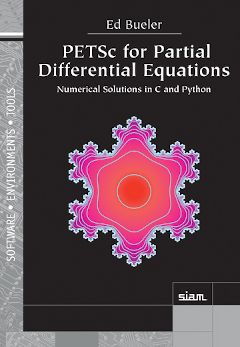
\includegraphics[width=15mm]{../talk-oxford/images/frontcover.jpg}
\end{frame}


\newcommand{\stacktwo}[2]{\begin{tabular}{c} #1 \\ #2 \end{tabular}}

\begin{frame}{multigrid strategies for VIs: feature table}

\begin{center}
\begin{tabular}{r|ccc}
   & \stacktwo{mesh-indep.}{rates}
       & \stacktwo{no need for}{global linearization}  \\ \hline
NM                         &              & \\
NM $+$ NI                  & $\checkmark$?& \\
{\color{FireBrick} FASCD}  & $\checkmark$ & $\checkmark$ {\Large \strut}
\end{tabular}
\end{center}


\medskip
{\small
\begin{center}
NM = Newton-multigrid, NI = nested iteration
\end{center}
}

\vspace{5mm}
\begin{itemize}
\item new algorithm (2023):

{\color{FireBrick} FASCD = full approximation scheme constraint decomposition}
\end{itemize}
\end{frame}


\subsection{full approximation scheme constraint decomposition (FASCD)}

\newcommand{\cK}{\mathcal{K}}

\begin{frame}{subspace decomposition}

\hfill 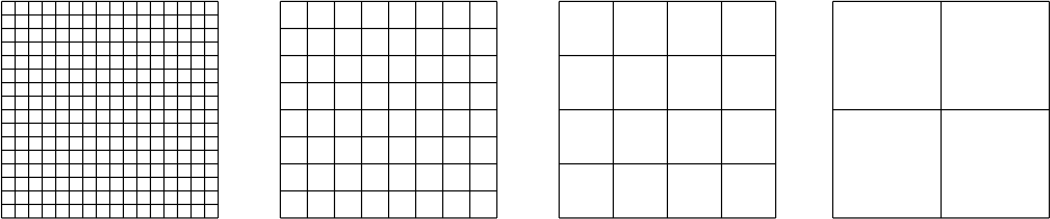
\includegraphics[height=0.12\textheight]{../talk-oxford/images/mg-grids.png}

{\footnotesize
\hfill $\Omega^3$ \hspace{8.5mm} $\Omega^2$ \hspace{8.5mm} $\Omega^1$ \hspace{8.5mm} $\Omega^0$ \hspace{1mm}
}

\begin{itemize}
\item to explain the ``CD'' (constraint decomposition) in FAS\underline{CD}, start with subspace decomposition in the multilevel case
\item assume mesh levels are nested: $\Omega^j \subset \Omega^{j+1}$ nodewise
\item let $\mathcal{V}^j$ be the space of FE functions on $\Omega^j$
    \begin{itemize}
    \item[$\circ$] standard FE spaces: \, $\mathcal{V}^j \subset \mathcal{V}^{j+1}$
    \end{itemize}
\begin{block}{definition}
$\ds \mathcal{V}^J = \sum_{i=0}^J \mathcal{V}^i$ \quad is called a \emph{subspace decomposition} (Xu 1992)
\end{block}
    \begin{itemize}
    \item[$\circ$] \emph{non}-unique vector space sum
    \end{itemize}
\end{itemize}
\end{frame}


\begin{frame}{constraint decomposition}

\begin{itemize}
\item Tai's (2003) constraint decomposition for VIs extends subspace decomposition to convex subsets
    \begin{itemize}
    \item[$\circ$] extends non-trivially
    \end{itemize}
\item suppose $\mathcal{K}^J \subset \mathcal{V}^J$ is a closed and convex subset
\item assume $\mathcal{V}^J = \sum_i\mathcal{V}^i$ is a subspace decomposition
\begin{block}{definition}
$\ds \mathcal{K}^J = \sum_{i=0}^J \mathcal{K}^i$ \quad is a \emph{constraint decomposition} (CD) if there are closed and convex subsets $\mathcal{K}^i\subset \mathcal{V}^i$, and (nonlinear) projections $\Pi_i : \mathcal{K}^J \to \mathcal{K}^i$, so that $\ds v = \sum_{i=0}^J \Pi_i v$ and a stability condition applies (not shown)
\end{block}
\end{itemize}
\end{frame}


\begin{frame}{constraint decomposition}

\begin{itemize}
\item observation: generally $\mathcal{K}^i \not\subset \mathcal{K}^J$
\item picture below: obstacle problem on a two-point mesh ($\mathcal{V} \cong \RR^2$)
\end{itemize}

\bigskip
\begin{center}
\includegraphics[width=0.6\textwidth]{../paper/genfigs/cartoon.pdf}
\end{center}
\end{frame}


\begin{frame}{constraint decomposition: multiplicative iterations}

\begin{itemize}
\item multiplicative iterations for $VI(F,\ell,\mathcal{K})$ over the CD

{\small
\begin{pseudo}[left-margin=-5mm]
\pr{cd-mult}(u)\text{:} \\+
    for $i = 0,\dots,m-1$: \\+
        find $w_i\in \cK_i$ s.t. \\+
            $\displaystyle \Big<f\Big(\sum_{j<i} w_j + w_i + \sum_{j>i} \Pi_j u\Big),\, v_i - w_i\Big> \ge \ip{\ell}{v_i - w_i} \,\forall v_i \in \cK_i$ \\--
    return $w=\sum_i w_i\in\cK$
\end{pseudo}
}
\end{itemize}
\end{frame}


\begin{frame}{defect obstacles}

\begin{itemize}
\item recall $\mathcal{K} = \{v \ge \psi\}$ in classical obstacle problem
\begin{block}{definition}
the \emph{defect obstacle} for a fine-level iterate $w^J \in \mathcal{K}^J = \{v\,:\,v\ge \psi^J\}$ is an FE function in $\mathcal{V}^J$:
    $$\chi^J = \psi^J - w^J$$
\end{block}
\item we generate the CD through defect obstacles $\chi^j$ on each level
\item via \emph{monotone restriction}: \quad $\ds \chi^j = R^{\oplus} \chi^{j+1}$
\end{itemize}

\begin{center}
\definecolor{seabornblue}{rgb}{0.2980392156862745, 0.4470588235294118, 0.6901960784313725}
\definecolor{seaborngreen}{rgb}{0.3333333333333333, 0.6588235294117647, 0.40784313725490196}
\definecolor{seabornred}{rgb}{0.7686274509803922, 0.3058823529411765, 0.3215686274509804}

\begin{tikzpicture}[scale=1.0]
  \foreach \k in {0, 1, 2, 3, 4} {
    %\filldraw[seabornblue, fill=seabornblue] ({cos(deg(2*\k*pi/5))}, {sin(deg(2*\k*pi/5))}) circle (1.5pt);
    \node (A) at ({0.5*cos(deg(2*\k*pi/5)) + 0.5*cos(deg(2*(\k+1)*pi/5))}, {0.5*sin(deg(2*\k*pi/5)) + 0.5*sin(deg(2*(\k+1)*pi/5))}) {};
    \node (B) at ({0.5*cos(deg(2*\k*pi/5))}, {0.5*sin(deg(2*\k*pi/5))}) {};
    \node (C) at ({0.5*cos(deg(2*(\k+1)*pi/5))}, {0.5*sin(deg(2*(\k+1)*pi/5))}) {};
    \node (D) at ({cos(deg(2*\k*pi/5))}, {sin(deg(2*\k*pi/5))}) {};
    \node (E) at ({cos(deg(2*(\k+1)*pi/5))}, {sin(deg(2*(\k+1)*pi/5))}) {};

    \draw [-,gray, very thick] (A.center) -- (B.center);
    \draw [-,gray, very thick] (B.center) -- (C.center);
    \draw [-,gray, very thick] (C.center) -- (A.center);

    \draw [black, ultra thick] (0, 0) -- (D.center);
    \draw [black, ultra thick] (D.center) -- (E.center);

    \filldraw[seaborngreen] (A) circle (1.5pt);
    \filldraw[seaborngreen] (B) circle (1.5pt);
    \filldraw[seaborngreen] (C) circle (1.5pt);
    \filldraw[seaborngreen] (D) circle (1.5pt);
    \filldraw[seaborngreen] (E) circle (1.5pt);

  }
  \filldraw[seabornblue] (0, 0) circle (2.5pt);
  
  \filldraw[seabornblue] (2.5, 0.5) circle (2.5pt);
  \node at (5.0, 0.5) {$= \text{coarse mesh node}$};
  \filldraw[seaborngreen] (2.5, 0.0) circle (1.5pt);
  \node (fine) at (4.5, 0.0) {$= \text{fine mesh node}$};
\end{tikzpicture}

\end{center}
\end{frame}


\begin{frame}{down and up sets}

\begin{itemize}
\item let $\mathcal{U}^j = \{z \ge \chi^j\}$, $\mathcal{D}^j = \{y \ge \phi^j=\chi^j - \chi^{j-1}\}$
\item get CD of fine-level constraint set:
	$$\mathcal{U}^J = \sum_{i=0}^J \mathcal{D}^i \phantom{KLDFJSKJDS SDF}$$
\end{itemize}

\begin{center}
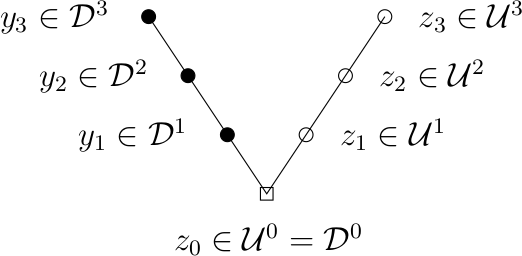
\includegraphics[width=0.4\textwidth]{../talk-oxford/images/fascd-vcycle.png}
\end{center}
\end{frame}


\begin{frame}{multilevel constraint decomposition}

\centering
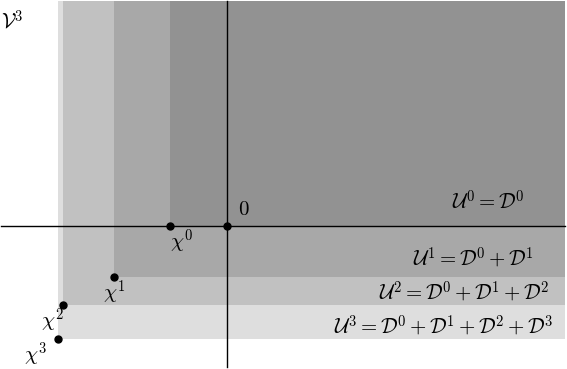
\includegraphics[width=0.7\textwidth]{figs/innerconeapprox.png}
\end{frame}


\begin{frame}{full approximation scheme constraint decomposition}

% case of lower obstacle only
\begin{pseudo}
\pr{fascd-vcycle}(J,\ell^J,\psi^J;w^J)\text{:} \\+
    $\chi^J = \psi^J - w^J$ \\
    for $j=J$ downto $j=1$ \\+
      $\chi^{j-1} = \maxR \chi^j$ \\
      $\phi^j = \chi^j - P\chi^{j-1}$ \\
      $y^j = 0$ \\
      $\text{\pr{smooth}}^{\text{\id{down}}}(\ell^j,\phi^j,w^j;y^j)$  \hspace{1.0cm} \ct{in $\mathcal{D}^j$}\\
      $w^{j-1} = \iR(w^j + y^j)$ \\
      $\ell^{j-1} = f^{j-1}(w^{j-1}) + R \left(\ell^j - f^j(w^j+y^j)\right)$ \\-
    $z^0 = 0$ \\
    $\text{\pr{solve}}(\ell^0,\chi^0,w^0;z^0)$ \hspace{1.0cm} \ct{in $\mathcal{U}^0$} \\
    for $j=1$ to $j=J$ \\+
      $z^j = y^{j} + P z^{j-1}$ \\
      $\text{\pr{smooth}}^{\text{\id{up}}}(\ell^j,\chi^j,w^j;z^j)$  \hspace{1.0cm} \ct{in $\mathcal{U}^j$} \\-
    return $w^J+z^J$
\end{pseudo}
\end{frame}


\section{results}

\subsection{classical obstacle problem}

\subsection{advection-diffusion of a concentration}

\subsection{glacier surface elevations}


\begin{frame}{classical obstacle problem}

\only<1>{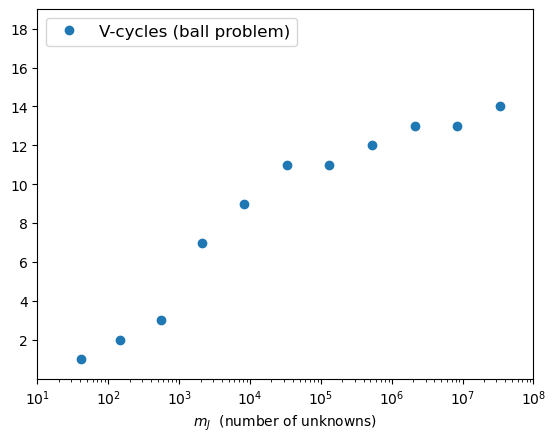
\includegraphics[width=0.75\textwidth]{figs/ballitersV.png}}\only<2>{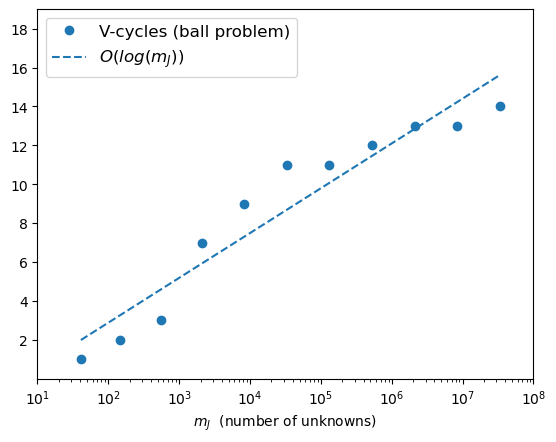
\includegraphics[width=0.75\textwidth]{figs/ballitersVlog.png}}\only<3>{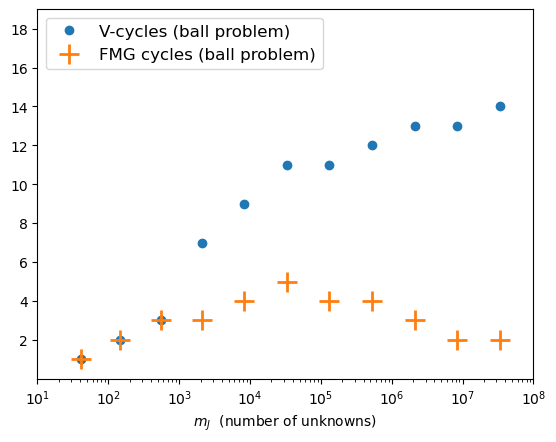
\includegraphics[width=0.75\textwidth]{figs/ballitersVF.png}}\only<4>{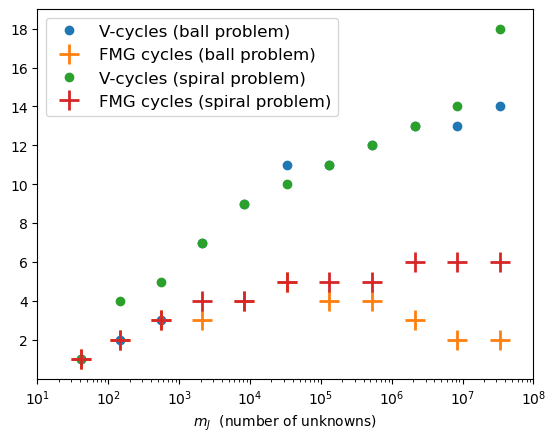
\includegraphics[width=0.75\textwidth]{figs/bothitersVF.png}} \hfill \only<1-3>{
\includegraphics[width=0.2\textwidth]{../paper/fixfigs/ball-set.png}}\only<4>{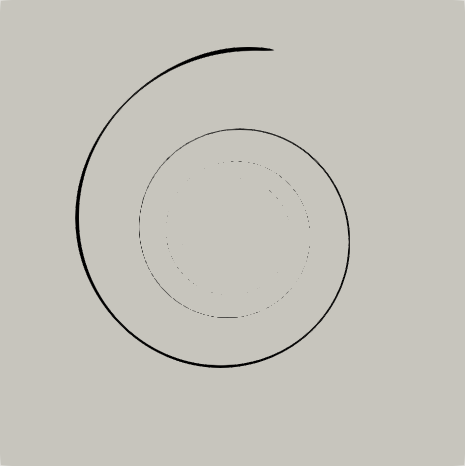
\includegraphics[width=0.2\textwidth]{../paper/fixfigs/spiral-set.png}}
\end{frame}


\begin{frame}{advection-diffusion of a concentration}

\mbox{

\includegraphics[width=0.3\textwidth]{../paper/fixfigs/poll2d-zero-set.png}
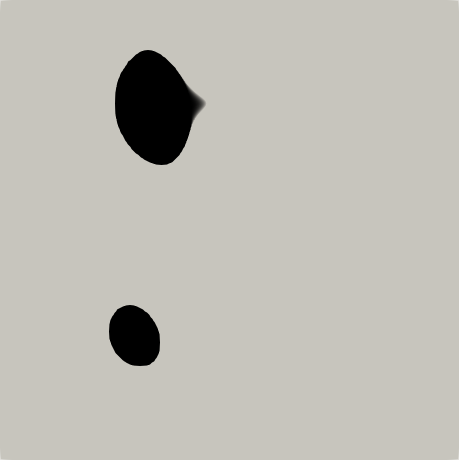
\includegraphics[width=0.3\textwidth]{../paper/fixfigs/poll2d-one-set.png}
}

\begin{itemize}
\item 2D problem: $-\eps \grad^2 u + \bm{X}\cdot \grad u = \phi$ with $0\le u\le 1$
\end{itemize}
\end{frame}


\begin{frame}{advection-diffusion of a concentration}

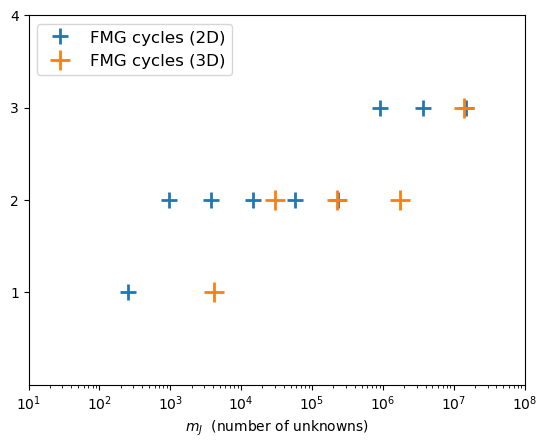
\includegraphics[width=0.75\textwidth]{figs/advdiff.png} \hfill \begin{minipage}[t]{0.2\textwidth}
\vspace{-50mm}


\includegraphics[width=\textwidth]{../paper/fixfigs/poll2d-zero-set.png}

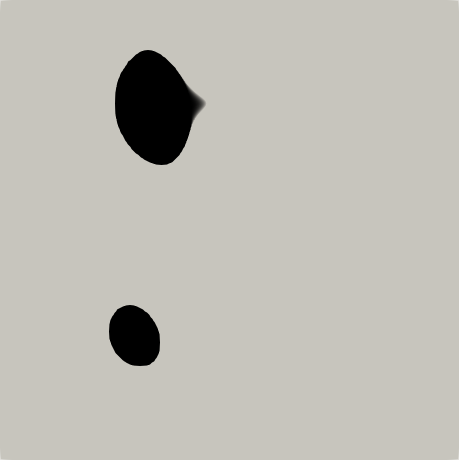
\includegraphics[width=\textwidth]{../paper/fixfigs/poll2d-one-set.png}
\end{minipage}
\end{frame}


\begin{frame}{problem: fluid layer in a climate}

\begin{itemize}
\item consider an incompressible, viscous layer with surface elevation $s(x,y)$, flowing with velocity $\bu(x,y,z)$, driven by gravity, over fixed bed topography with elevation $b(x,y)$, in a \emph{climate} which adds or removes fluid at a signed rate $a(x,y)$ [$\text{m}\,\text{s}^{-1}$]
    \begin{itemize}
    \item[$\circ$] data $a,b$ defined on domain $\Omega \subset \RR^2$
    \end{itemize}
\item geophysical examples: \alert{glaciers and ice sheets}, sea ice, lakes
\end{itemize}

\bigskip
\hfill \mbox{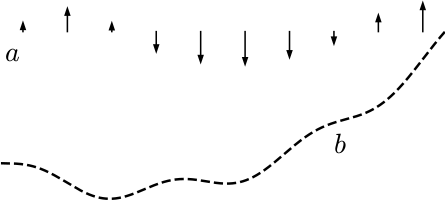
\includegraphics[height=0.25\textheight]{../talk-oxford/images/domain-data.png} \hspace{7mm} 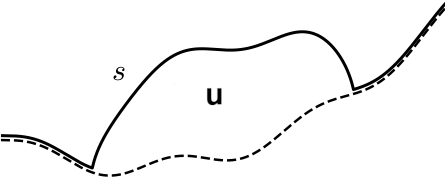
\includegraphics[height=0.25\textheight]{../talk-oxford/images/domain-velocity.png}}
\end{frame}


\begin{frame}{example: glacier ice coverage of the Alps in prior climates}

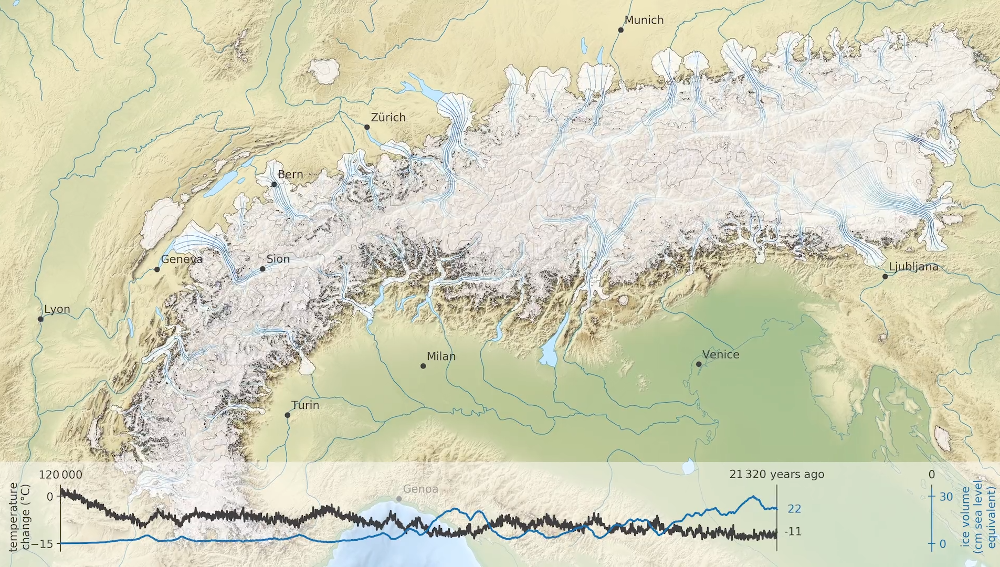
\includegraphics[width=1.02\textwidth]{../talk-oxford/images/alps-seguinot2018.png}

\vspace{-2mm}
\hfill {\tiny Sequinot et al.~(2018)}
\end{frame}


\begin{frame}{naive strong form}

\begin{itemize}
\item naive strong form of the steady model: % ($\bn_s = \left<-s_x,-s_y,1\right>$ is surface normal):
\begin{align*}
s &\ge b                    & &\text{everywhere in } \Omega \\
-\bu|_s \cdot \bn_s &= a    & &\text{where } s(x,y) > b(x,y)
\end{align*}

    \begin{itemize}
    \item[$\circ$] surface velocity $\bu|_s$ is determined by fluid domain geometry $s$
    \item[$\circ$] $\bn_s=\left<-\grad s,1\right>$ is upward surface normal
    \item[$\circ$] generally: $-\bu|_s \cdot \bn_s$ is a \emph{non-local} function of $s$
    \end{itemize}
\item the inequality constraint $s \ge b$ \alert{generates a free boundary}

if an ablative climate $a < 0$ forces surface down to bed
\end{itemize}

\bigskip
\hfill \mbox{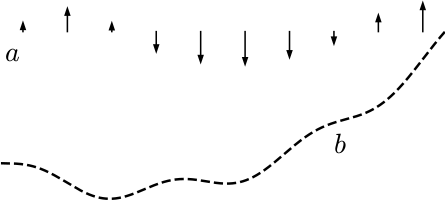
\includegraphics[height=0.2\textheight]{../talk-oxford/images/domain-data.png} \hspace{7mm} 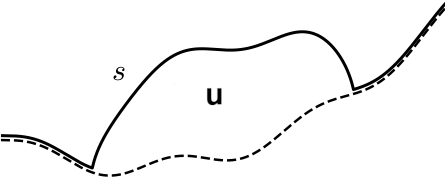
\includegraphics[height=0.2\textheight]{../talk-oxford/images/domain-velocity.png}}
\end{frame}


\begin{frame}{shallow ice approximation}

\begin{itemize}
\item with enough simplifications we may compute the surface motion term by applying a nonlinear elliptic differential operator to $s$:
    $$\Phi(s) = - \frac{\gamma}{\qq} (s-b)^{\qq} |\grad s|^{\qq} - \grad \cdot\left(\frac{\gamma}{\qq+1} (s-b)^{\qq+1} |\grad s|^{\qq-2} \grad s\right)$$
    \begin{itemize}
    \item $\qq = 4$
    \item $\grad$ is in $x,y$ only
    \item $\Phi(s)$ is a nonlinear \alert{differential operator} in this model because membrane stresses are \emph{not} balanced
    \item $\Phi(s)$ is doubly-degenerate
    \end{itemize}
\end{itemize}
\end{frame}


\begin{frame}{VI for fluid layer in a climate}

\begin{itemize}
\item admissible surface elevations:
    $$\mathcal{K} = \left\{r \in \mathcal{V} \,:\, r \ge b\right\}$$

    \begin{itemize}
    \item[$\circ$] $\mathcal{V}$ to be determined by viscous fluid model\footnote{in shallow ice approximation, $(s-b)^{8/3} \in W^{1,4}(\Omega)$ (Jouvet \& Bueler, 2012)}
    \end{itemize}
\item VI problem for surface elevation $s\in\mathcal{K}$:
	$$\ip{\Phi(s)}{r-s} \ge \ip{a}{r-s} \quad \text{ for all } r \in \mathcal{K}$$
where
    $$\Phi(s)=- \bu|_s \cdot \bn_s,$$
with extension by 0 to all of $\Omega$, and $\bu$ is the velocity solution on
    $$\Lambda(s) = \{(x,y,z) : b(x,y) < z < s(x,y)\}$$
\end{itemize}
\end{frame}


\begin{frame}{computed ice sheet}

\centering
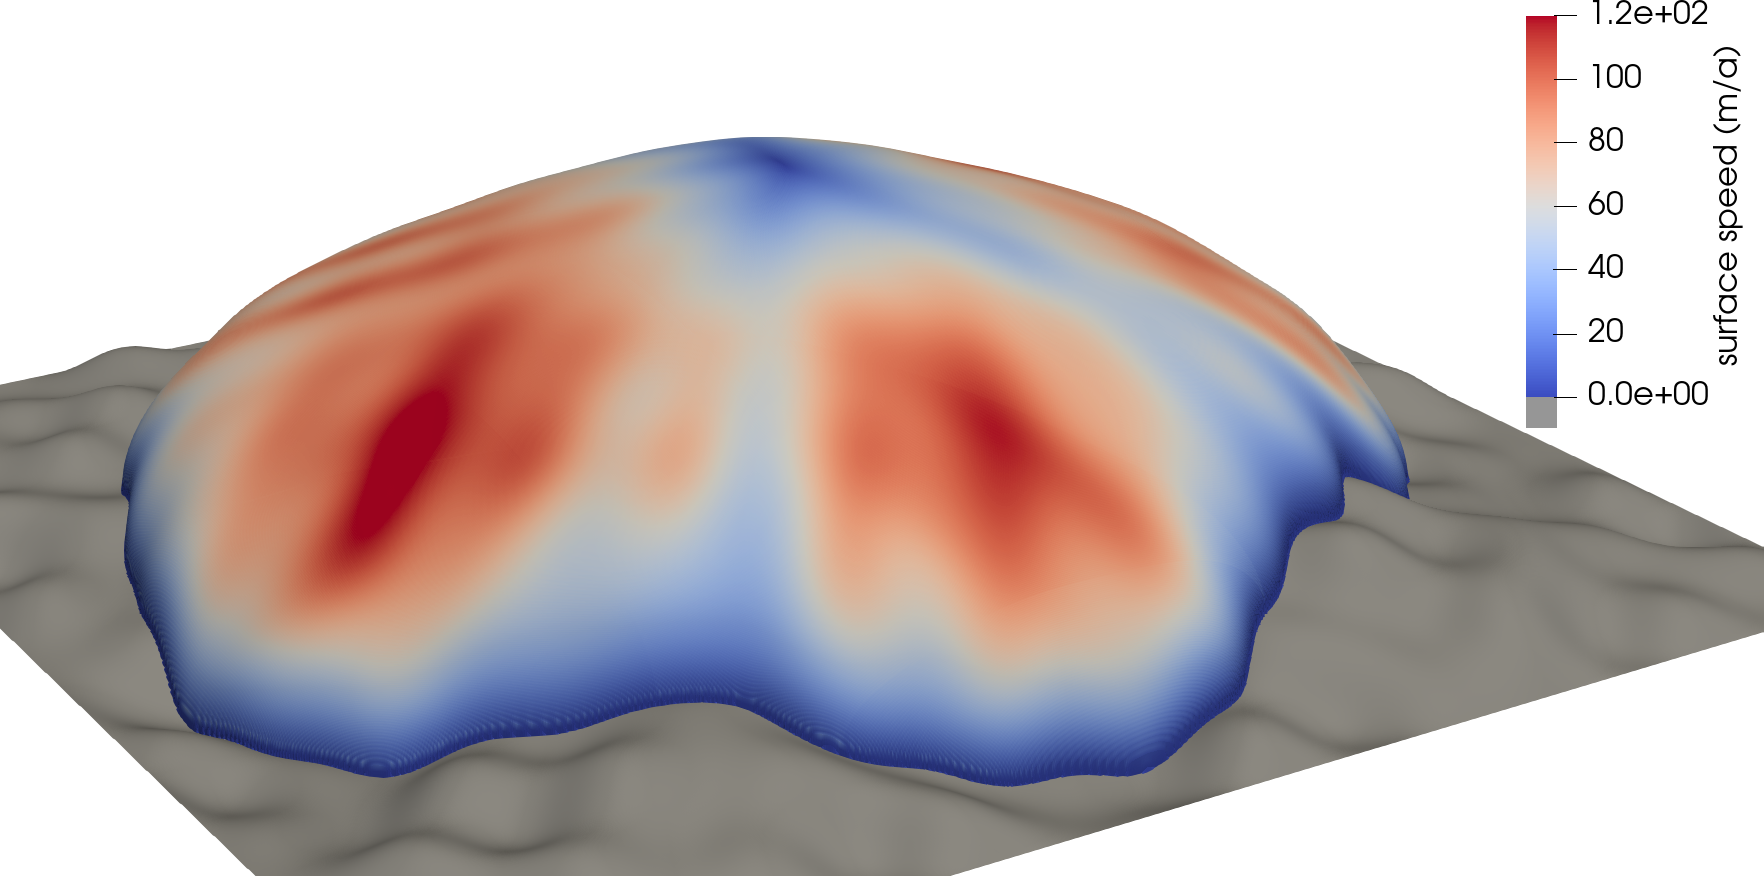
\includegraphics[width=\textwidth]{../paper/fixfigs/sialev8scene.png}

FIXME ice sheet the size of Greenland
\end{frame}


\begin{frame}{weak-scaling}

\centering
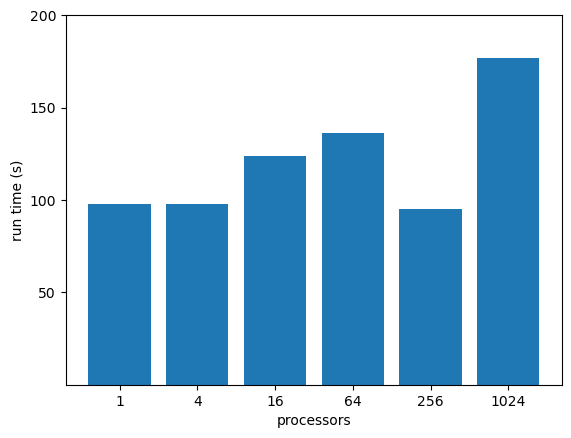
\includegraphics[width=0.7\textwidth]{figs/siaweaktime.png}

FIXME final run had $m_J=20481^2=4.1\times 10^8$ unknowns and a 88 meter grid resolution
\end{frame}


\begin{frame}{summary and outlook}

\begin{itemize}
\item FIXME
\end{itemize}
\end{frame}


\begin{frame}{references}

%{\scriptsize
{\notsotiny
% inputed at end of slides.tex

\newcommand{\sdoi}[1]{\,{\tiny \href{https://doi.org/#1}{doi:#1}}}
\begin{itemize}
\item A.~Brandt \& C.~Cryer (1983). \emph{Multigrid algorithms for the solution of linear complementarity problems \dots}, SIAM J.~Sci.~Stat.~Comput.~4 (4), 655--684 \sdoi{10.1137/0904046}
%FTITLE Multigrid algorithms for the solution of linear complementarity problems arising from free boundary problems
\item P.~Brune, M.~Knepley, B.~Smith, \& X.~Tu (2015). \emph{Composing scalable nonlinear algebraic solvers}, SIAM Review~57 (4), 535--565 \sdoi{10.1137/130936725}
\item E.~Bueler (2021). \emph{Conservation laws for free-boundary fluid layers}, SIAM J.~Appl.~Math.~81 (5), 2007--2032 \sdoi{10.1137/20M135217X}
%\item E.~Bueler (2022). \emph{Performance analysis of high-resolution ice-sheet simulations}, J.~Glaciol., \sdoi{10.1017/jog.2022.113}
\item G.~de Diego, P.~Farrell, \& I.~Hewitt (2022). \emph{Numerical approximation of viscous contact problems applied to glacial sliding}, J.~Fluid Mech.~938 (A21). \sdoi{10.1017/jfm.2022.178}
\item P.~Farrell, M.~Croci, \& T.~Surowiec (2020). \emph{Deflation for semismooth equations}, Optimization Methods \& Software 35 (6), 1248--1271 \sdoi{10.1080/10556788.2019.1613655}
\item C.~Gr{\"a}ser \& R.~Kornhuber (2009). \emph{Multigrid methods for obstacle problems}, J.~Comput.~Math., 1--44
\item T.~Isaac, G.~Stadler, \& O.~Ghattas (2015). \emph{Solution of nonlinear Stokes equations \dots ice sheet dynamics}, SIAM J.~Sci.~Comput., 37 (6), B804--B833 \sdoi{10.1137/140974407}
%FTITLE Solution of nonlinear Stokes equations discretized by high-order finite elements on nonconforming and anisotropic meshes, with application to ice sheet dynamics
\item G.~Jouvet \& E.~Bueler (2012). \emph{Steady, shallow ice sheets as obstacle problems \dots}, SIAM J.~Appl.~Math.~72 (4), 1292--1314 \sdoi{10.1137/110856654}
%FTITLE Steady, shallow ice sheets as obstacle problems: well-posedness and finite element approximation
\item G.~Jouvet \& J.~Rappaz (2011). \emph{Analysis and finite element approximation of a nonlinear stationary {S}tokes problem \dots}, Adv.~Numer.~Analysis 2011 (164581) \sdoi{10.1155/2011/164581}
%FTITLE Analysis and finite element approximation of a nonlinear stationary {S}tokes problem arising in glaciology
\item R.~Kornhuber (1994). \emph{Monotone multigrid methods for elliptic variational inequalities I}, Numer.~Math.~69, 167--184 \sdoi{10.1007/BF03325426}
\item A.~Reusken (1987). \emph{Convergence of the multigrid full approximation scheme \dots}, Numer.~Math.~52, 251--277 \sdoi{10.1007/BF01398879}
%FTITLE Convergence of the multigrid full approximation scheme for a class of elliptic mildly nonlinear boundary value problems
\item J.~Seguinot \& 5 others (2018).  \emph{Modelling last glacial cycle ice dynamics in the Alps}, The Cryosphere, 12 (10), 3265--3285 \sdoi{10.5194/tc-12-3265-2018}
%FAUTHORS Seguinot, J., Ivy-Ochs, S., Jouvet, G., Huss, M., Funk, M., & Preusser, F.
\item X.~Tai (2003). \emph{Rate of convergence for some constraint decomposition methods for nonlinear variational inequalities}, Numer.~Math.~93 (4), 755--786 \sdoi{10.1007/s002110200404}
\end{itemize}


}
\end{frame}

\begin{frame}{background references}

%{\scriptsize
{\notsotiny
% inputed at end of slides.tex

\newcommand{\sdoi}[1]{\,{\tiny \href{https://doi.org/#1}{doi:#1}}}
\begin{itemize}
\item E.~Bueler (2021). \emph{PETSc for Partial Differential Equations}, SIAM Press, Philadelphia
\item N.~Kikuchi \& J.~Oden (1988).  \emph{Contact Problems in Elasticity: A Study of Variational Inequalities and Finite Element Methods}, SIAM Press, Philadelphia
\item D.~Kinderlehrer \& G.~Stampacchia (1980). \emph{An Introduction to Variational Inequalities and their Applications}, Academic Press, New York
\item U.~Trottenberg, C.~Oosterlee, \& A. Schuller (2001).  \emph{Multigrid}, Elsevier, Oxford
\end{itemize}


}
\end{frame}

\end{document}
